\documentclass[man,noapacite]{apa2}
\usepackage{amsmath}
\usepackage{booktabs}
\usepackage{apacite2}
\usepackage{fullpage,rotating}
\usepackage{pslatex}
\usepackage{amssymb}
% \usepackage{synctex}

\title{Learning word meaning by inferring speakers' intended referents: \\ An incremental approach to socially-guided statistical learning}

\threeauthors{Michael C. Frank}{Molly L. Lewis}{Noah D. Goodman}
\threeaffiliations{Department of Psychology, Stanford University}{Department of Psychology, Stanford University}{Department of Psychology, Stanford University}

\shorttitle{Learning words by inferring reference}
\rightheader{Learning words by inferring reference}


\acknowledgements{Many thanks to ...

~

\noindent Please address correspondence to Michael C. Frank, Department of Psychology, Stanford University, 450 Serra Mall (Jordan Hall), Stanford, CA, 94305, tel: (650) 724-4003, email: \texttt{mcfrank@stanford.edu}.}


\abstract{How do children learn word meanings?}

\begin{document}
\maketitle                            


\section{Introduction}


\section{Model}

\subsection{Model Specification}
\begin{figure}[tr]
\begin{center}
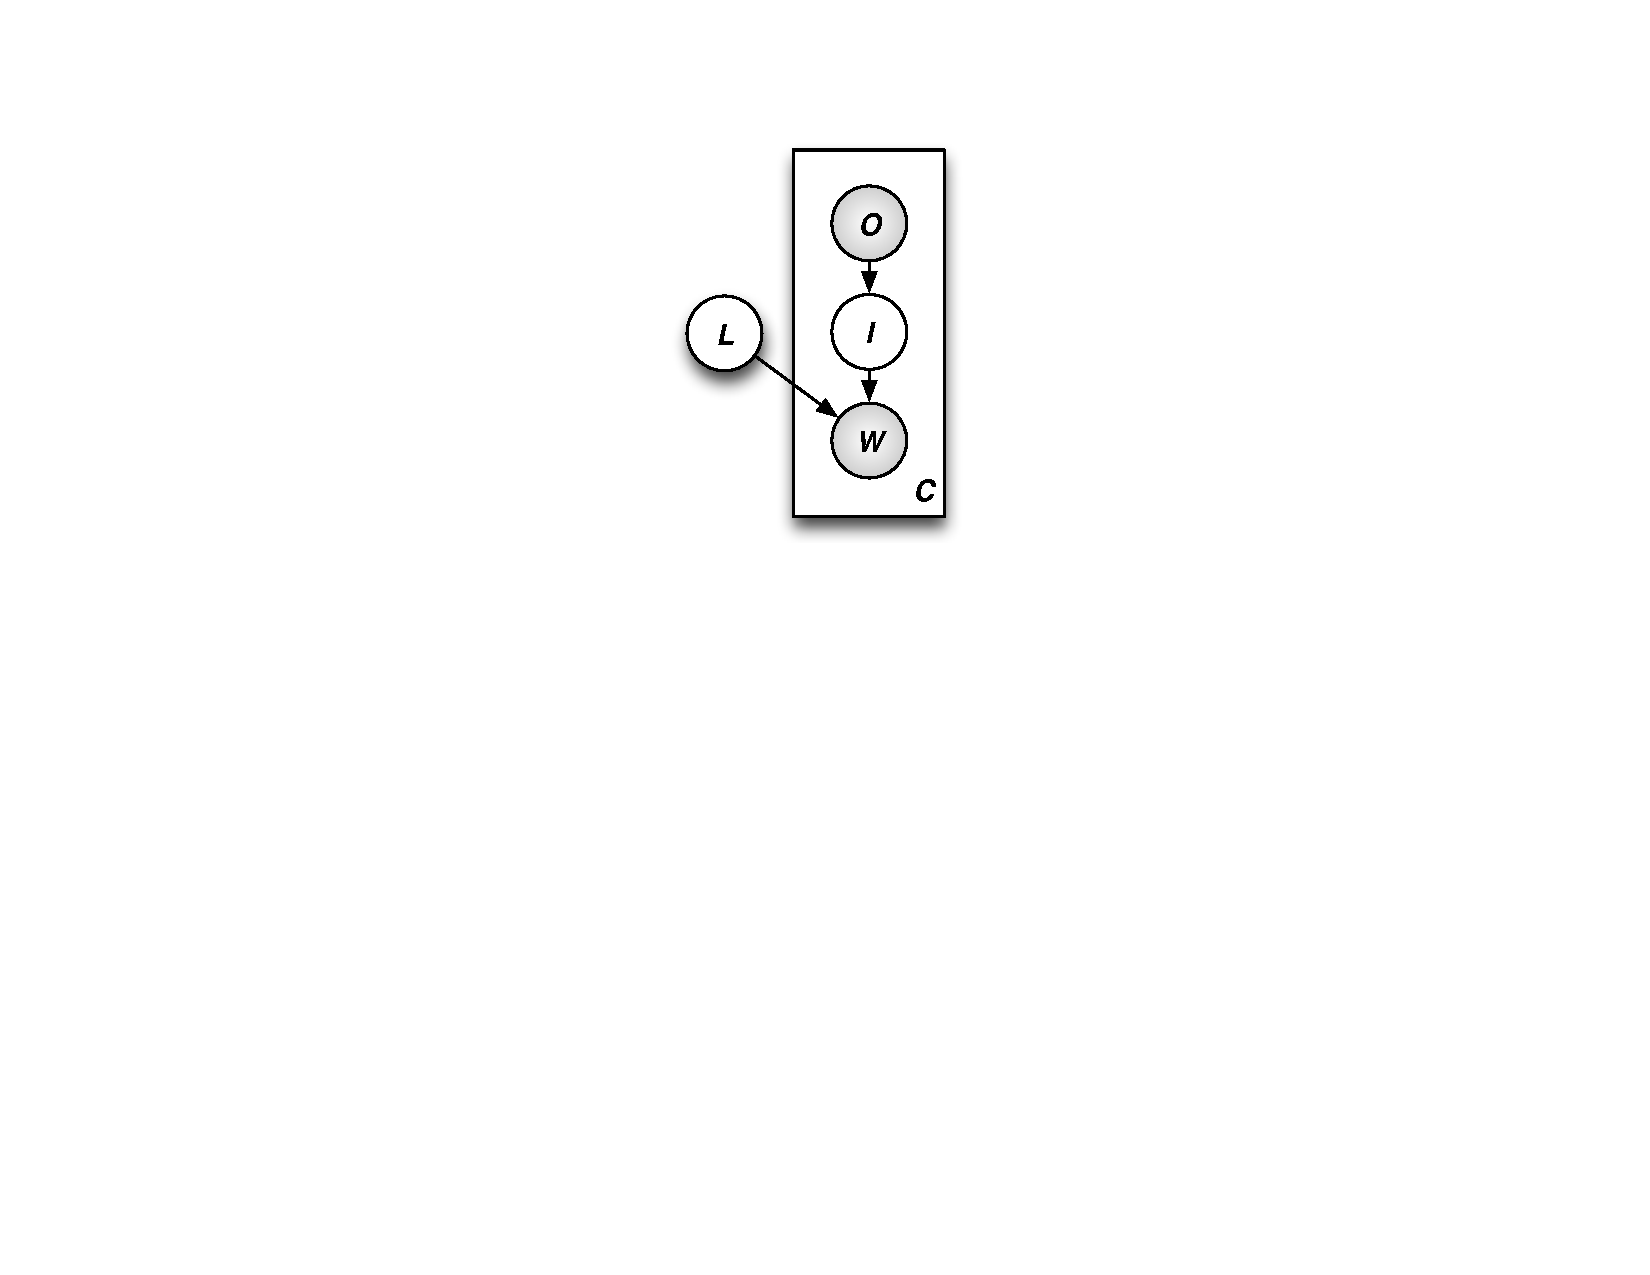
\includegraphics[width=1.5in]{figures/gen_mod.pdf}
\caption{\label{fig:genmod} Caption.}
\end{center}
\end{figure}

\begin{figure}[tr]
\begin{center}
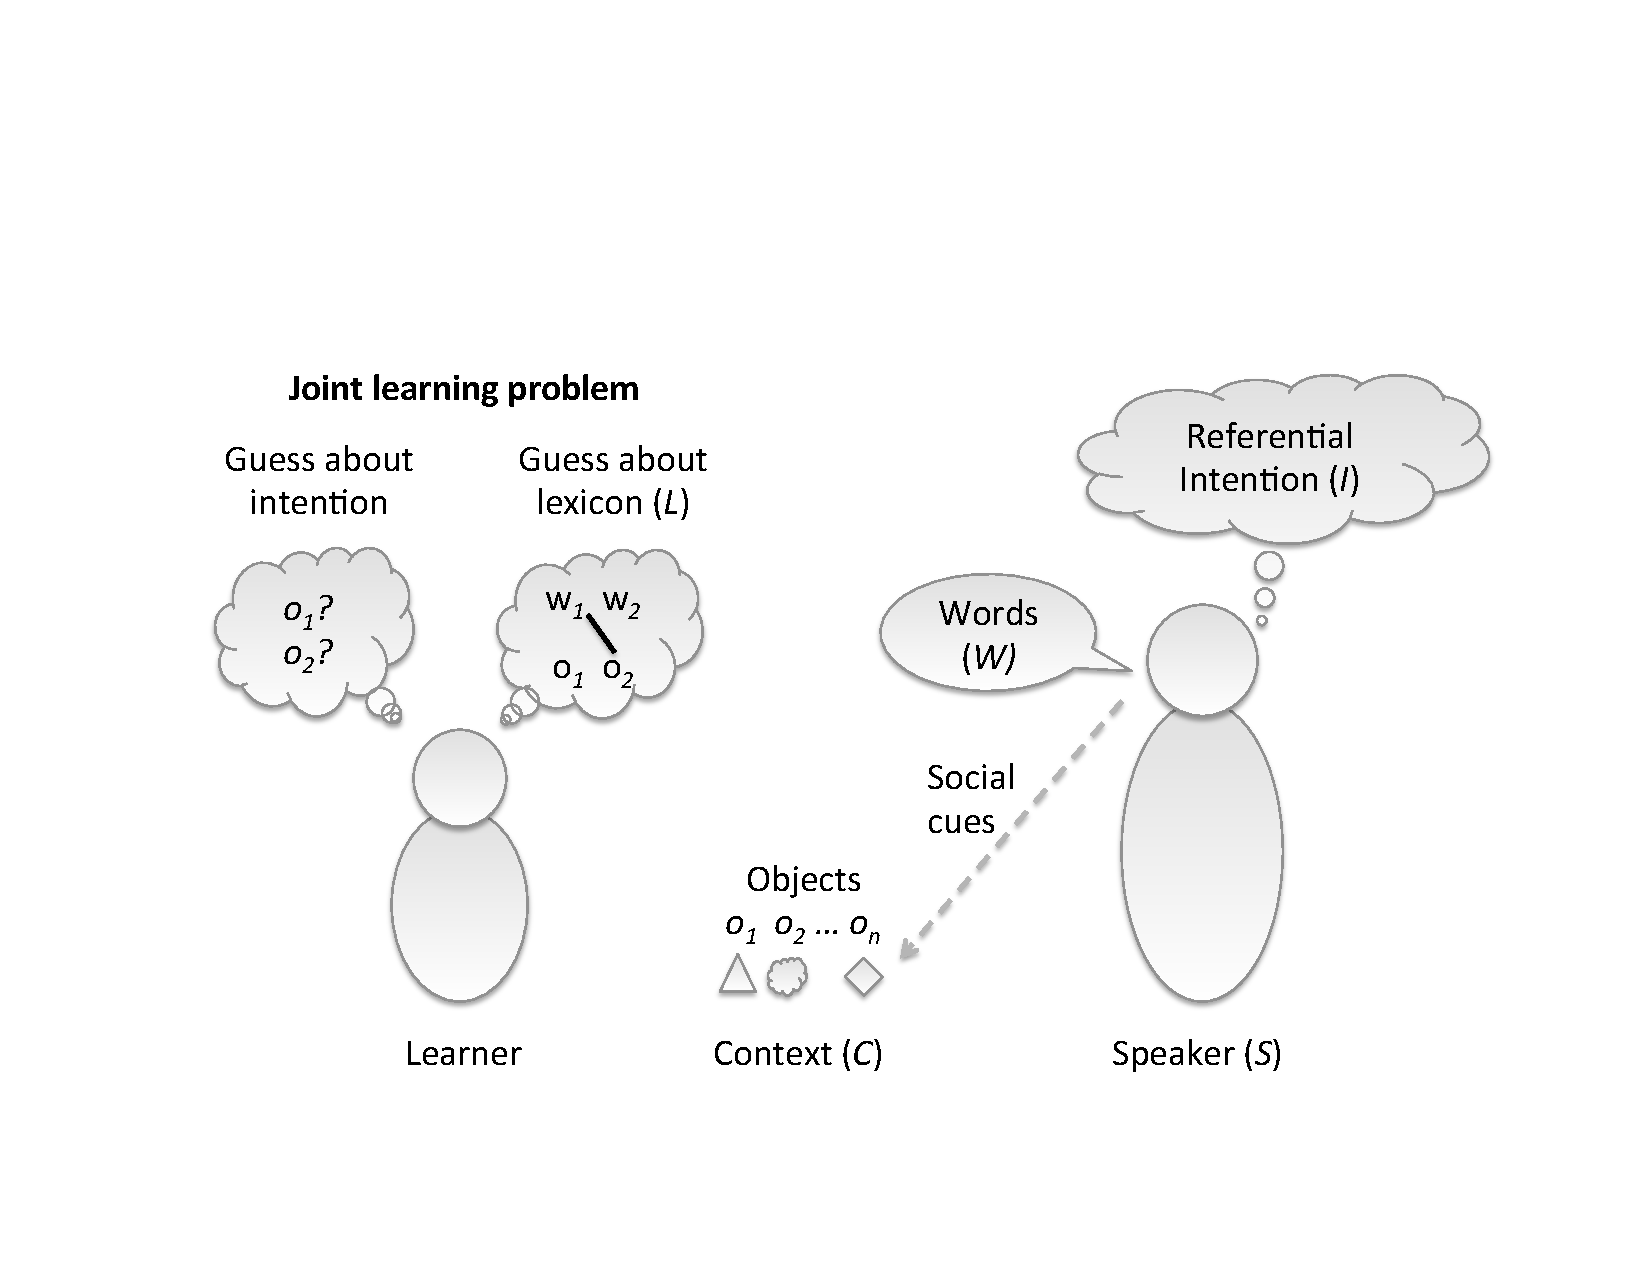
\includegraphics[width=4.5in]{figures/setup.pdf}
\caption{\label{fig:setup} Caption. From Frank (in press). }
\end{center}
\end{figure}

By Bayes' rule:

\begin{equation}
P( I| C) \propto P(C | I) P(I).
\end{equation}


\begin{equation}
P( I| W, O) \propto P(W | I, O) P(I).
\end{equation}

\noindent But the objects $O$ are observed in the context. In addition, for simplicity, we assume that there is a uniform prior over possible intentions (though we return to this issue in the Discussion). By the generative model in Figure \ref{fig:genmod}, the remaining expression can be factored as follows:

\begin{equation}
P( I| W, O, L) \propto P(W | I, L) P(I | O) P(L).
\end{equation}

But now we integrate over all possible L:

\begin{equation}
P( I| W, O, L) \propto \int_L{P(W | I, L) P(I | O) P(L)}
\end{equation}


In this model, the lexicon $L$ consists of two separate parts. The referential lexicon $L_R$ is a set of integrated Dirichlet-Multinomial distributions, one for each object in the world. This distribution represents the posterior probability of a particular word, relative to that object. 

\begin{equation}
P(L) = \prod{o \in W}{P(L_o)} + P(L_{NR}).
\end{equation}

 

\begin{equation}
P(W | I, L) = \gamma  
\end{equation}


\subsection{Inference}
\begin{figure}[tr]
\begin{center}
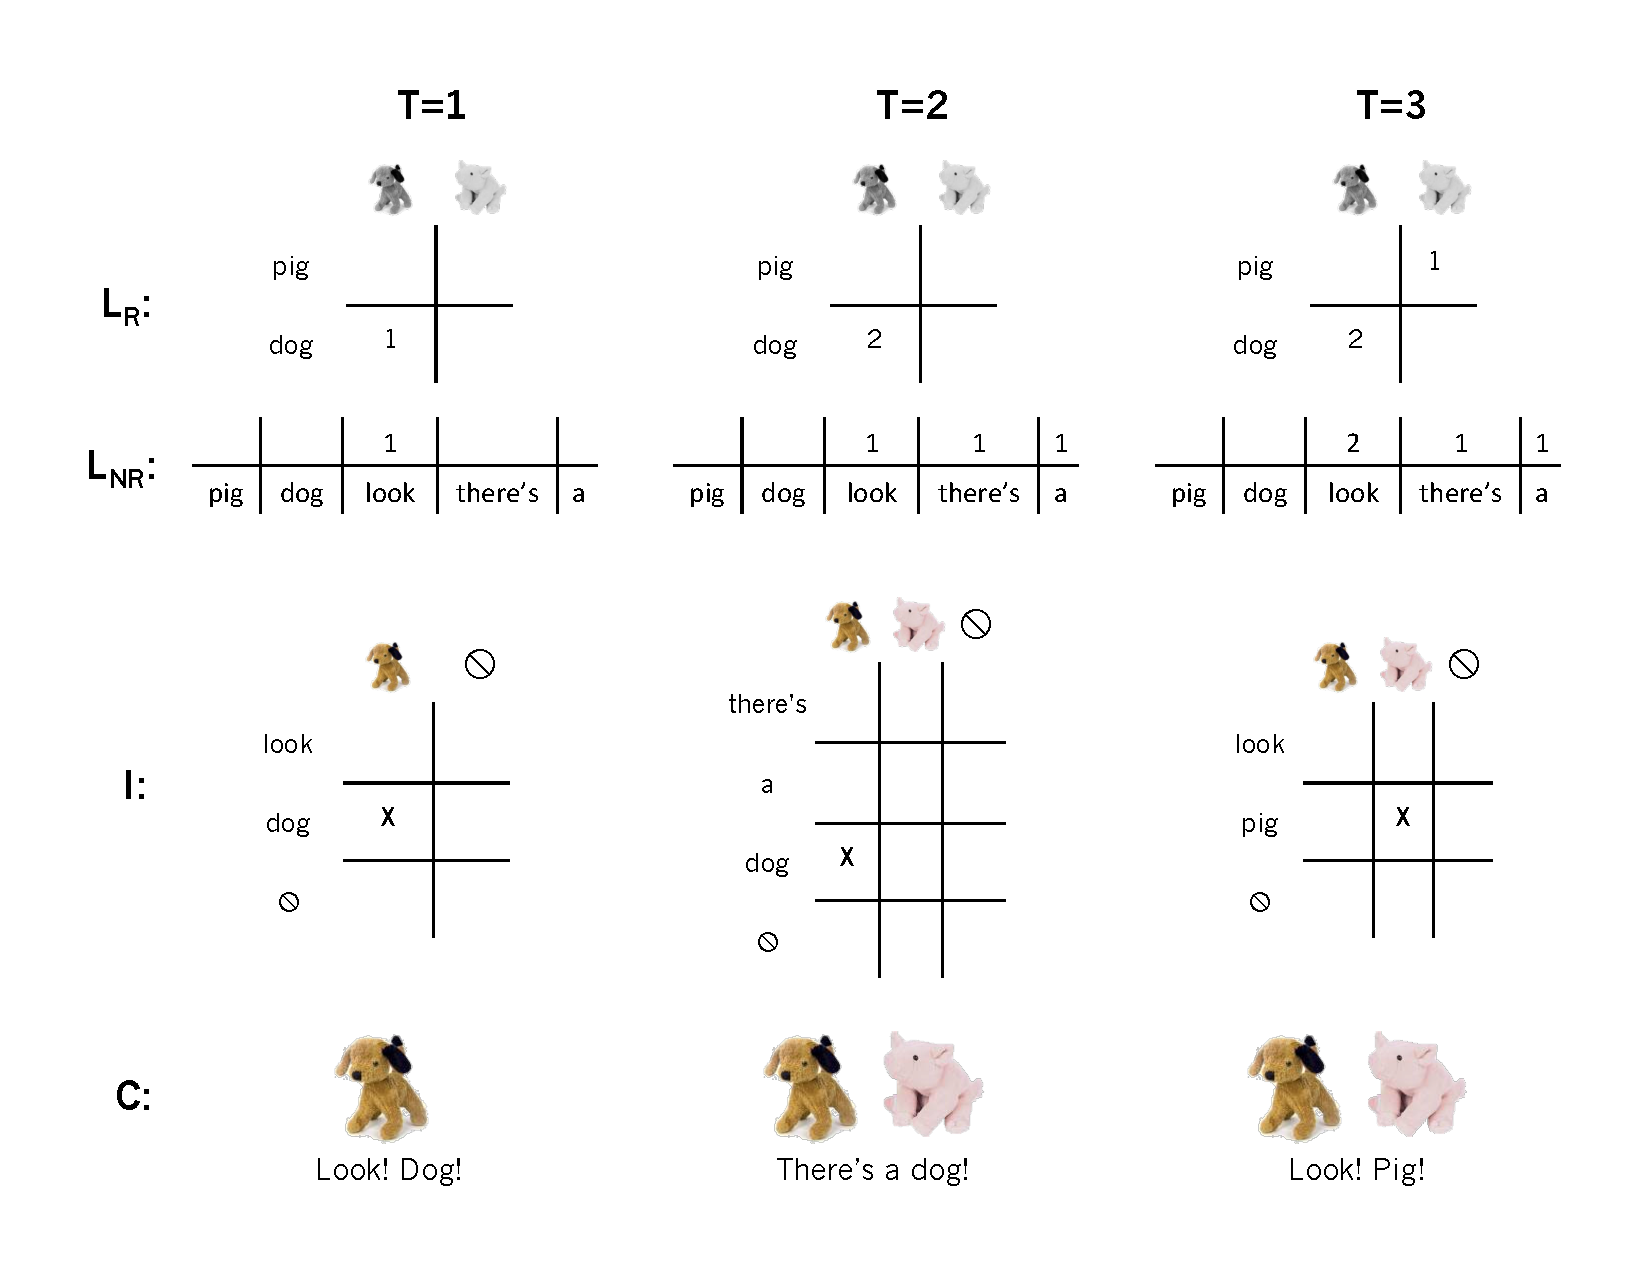
\includegraphics[width=6.5in]{figures/inference_diagram.pdf}
\caption{\label{fig:inference_diagram} Caption.}
\end{center}
\end{figure}

\subsubsection{Batch inference using a gibbs sampler}

\subsubsection{Incremental inference using a particle filter}

\section{Simulations}

\subsection{Cross-situational word learning with adults}

\subsubsection{Yu \& Smith (2007)}

\subsection{Experiments with children}

\subsubsection{Disambiguation}

\subsubsection{Dewar \& Xu (2007)}


\subsection{Corpus simulations}

\subsection{Rollins subset (Frank, Goodman, \& Tenenbaum, 2009)}

\subsection{Fernald \& Morikawa (Johnson, Demuth, \& Frank, 2012)}

\section{Discussion}

\newpage

\bibliographystyle{apacite}
\bibliography{icom}

\end{document}

